\section{Cycle-shedding demonstration}
\label{app:cycle-shedding-demonstration}

\subsection{Scope}
\label{app:cycle-shedding-demo-scope}
This demonstration run illustrates boundary accounting after the ontology has been declared. It uses one temporal cycle group on one retained field and records lead--lag span, temporal SADAR burden, sheddic excess, outward remainder, local reclosure, and sheddic path triggers.

\subsection{Setup}
\label{app:cycle-shedding-demo-setup}
For update index \(t\), let \(L_t\) be the lead component, \(G_t\) the lag component, \(S_t\) the disturbance span, \(P_t\) the burden, \(C_t\) local closure compatibility, \(X_t\) sheddic excess, \(O_t\) outward remainder, and \(R_t\) local reclosure.

\subsection{Statement(s)}
\label{app:cycle-shedding-demo-statements}
\[
S_t=|L_t-G_t|,
\qquad
\widetilde P_t=\eta_{\mathrm{ret}} P_{t-1}+\gamma_{\mathrm{span}} S_t,
\]
\[
X_t=\max(0,\widetilde P_t-C_t),
\qquad
P_t=\widetilde P_t-X_t,
\]
\[
O_t=(1-\lambda_{\mathrm{reclose}})X_t,
\qquad
R_t=\lambda_{\mathrm{reclose}}X_t.
\]
Here \(O_t\) is the non-reclosed outward remainder; route placement may later split it into exoshedding, redirected support routing, and open loss.

\subsection{Demonstration}
\label{app:cycle-shedding-demo-demonstration}
The displayed run uses \(90\) update steps, retention coefficient \(\eta_{\mathrm{ret}}=41/50\), span gain \(\gamma_{\mathrm{span}}=11/20\), and reclosure fraction \(\lambda_{\mathrm{reclose}}=19/50\). The lead and lag components are declared deterministic test streams with two local disturbance pulses.

\begin{figure}[H]
\centering
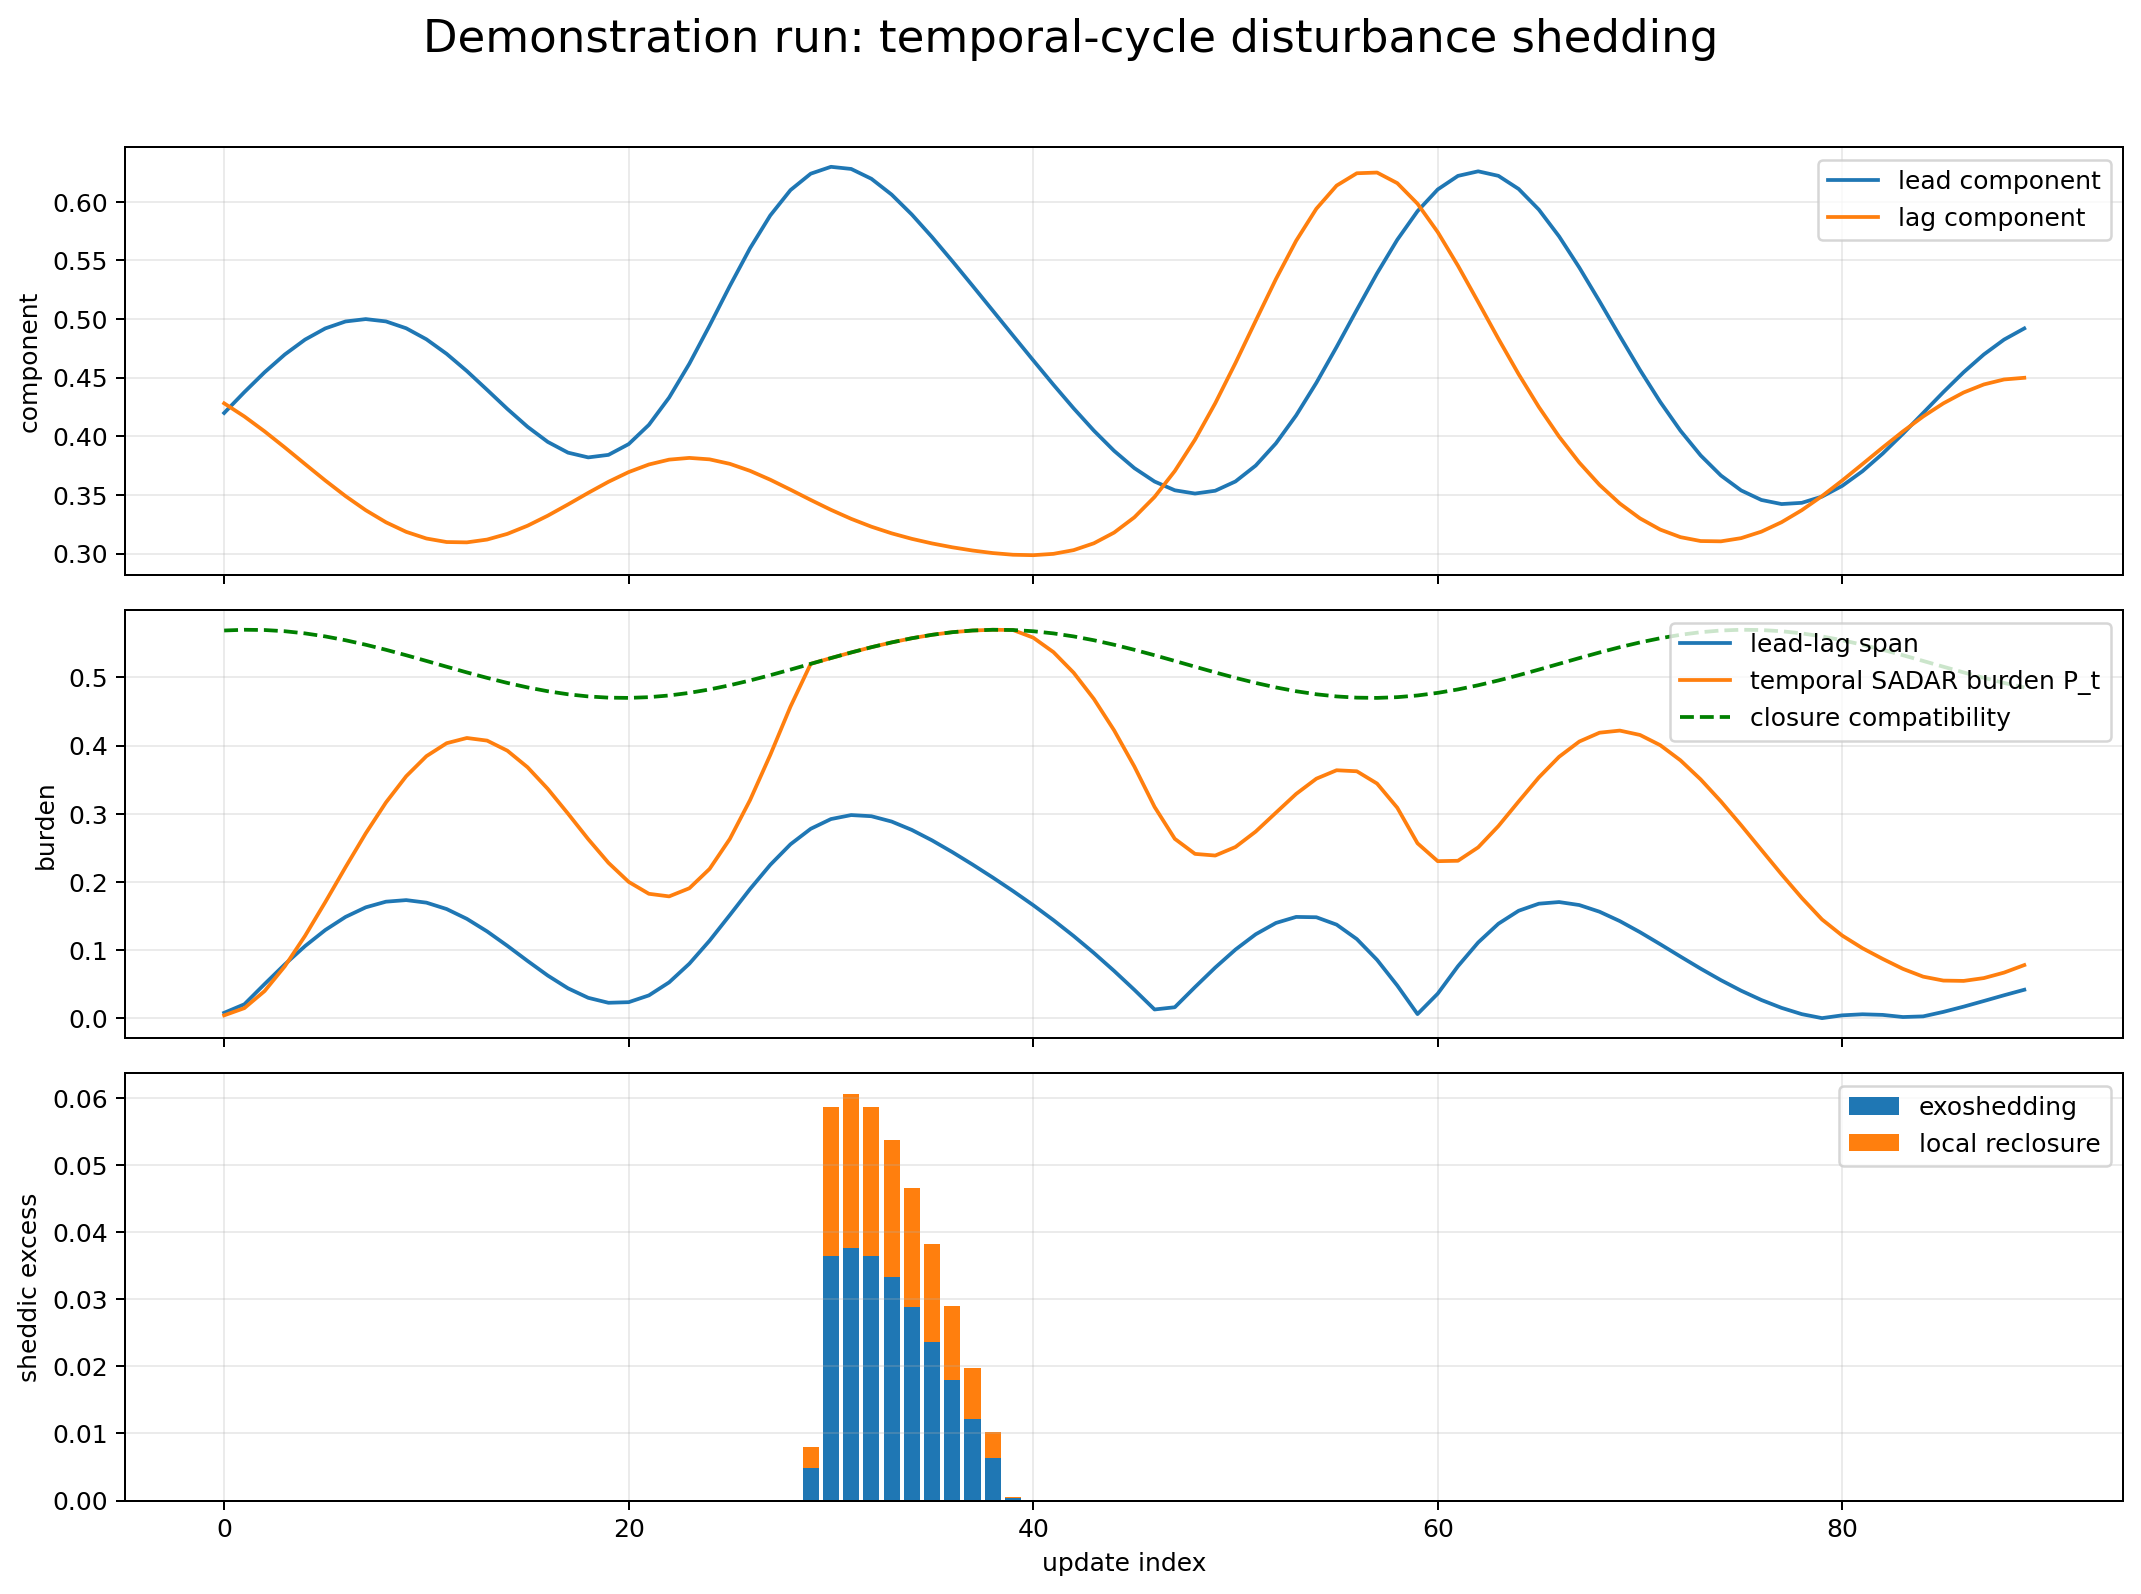
\includegraphics[width=0.98\linewidth]{figures_jpg/cycle_disturbance_shedding_simulation.png}
\caption{Demonstration run: temporal-cycle disturbance shedding.}
\label{fig:v39-cycle-shedding-simulation}
\end{figure}

\begin{center}
\begin{tabular}{lr}
\toprule
Ticks & 90 \\
Maximum lead-lag span & 0.298 \\
Maximum temporal SADAR burden & 0.570 \\
Maximum sheddic excess & 0.061 \\
Total exoshedding & 0.238 \\
Total local reclosure & 0.146 \\
Sheddic path trigger ticks & 0 \\
First reclosure tick & none \\
\bottomrule
\end{tabular}

\end{center}

\subsection{Falsification}
\label{app:cycle-shedding-demo-falsification}
If the computed values violate the stated recurrences on the declared update indices, the demonstration fails on that run.

\aodprovenance{\secref{subsec:temporal-sadar-burden},
\secref{subsec:shedding},
\secref{subsec:sheddic-path}.}
